\documentclass[10pt]{article}
\usepackage[T1]{fontenc}
\usepackage{amsmath,amssymb}
\usepackage{booktabs}
\usepackage{graphicx}
\usepackage[table]{xcolor}
\usepackage{tikz}
\usetikzlibrary{positioning,arrows.meta}
\usepackage[font=small,labelfont=bf]{caption}
% Standalone preview only; drop when pasting into the organizers' template.
\usepackage[margin=1in]{geometry}

\graphicspath{{figures/}}
\definecolor{cblue}{HTML}{2A78D6}
\definecolor{cred}{HTML}{E34948}
\definecolor{cgray}{HTML}{52514E}
\definecolor{cbase}{HTML}{EEF4FC}
\newcommand{\dpos}[1]{\textcolor{cblue}{\footnotesize(#1)}}
\newcommand{\dneg}[1]{\textcolor{cred}{\footnotesize(#1)}}

\title{\Large Can a Normal Universe Explain This Map?\\[3pt]
\large Out-of-Distribution Detection for Weak Lensing by Misfit, Consistency and Outlier Exposure}
\author{Sachin Konan}
\date{}

\begin{document}
\maketitle

\begin{abstract}
I detect weak-lensing convergence maps that the simulator did not produce. My starting observation is that
normal maps differ mostly because they come from different universes: a detector that ignores the five generating
parameters barely beats chance on my synthetic distortions, while the same statistics, told the true parameters,
detect them well. I therefore ask of each test map whether \emph{some} normal universe can explain it. Three tests
answer this: the misfit left after fitting the parameters, the disagreement between parameters fitted from
different views of the map, and a classifier trained to recognize distorted maps. Their calibrated scores are
averaged. The method scores 0.7037 on the public leaderboard, up from 0.5253 for the pipeline I started from, and
scores the 10,000 test maps in about five minutes on one GPU.
\end{abstract}

% =================================================================================================
\section{Introduction}

A weak-lensing analysis reads cosmology off the matter distribution by comparing observed convergence maps with
simulated ones. The comparison is only as good as the simulator. A map shaped by physics or systematics the
simulator leaves out --- an unmodeled baryonic effect, intrinsic alignments, a PSF residual --- will still be fitted,
and will quietly bias the inferred parameters. Phase~2 of the FAIR Universe challenge asks for the step that should
come first: flag such maps.

The task is easy to state. The training set holds 25,856 simulated maps, each paired with the five parameters that
generated it: $\theta=(\Omega_m, S_8, T_{\mathrm{AGN}}, f_0, \Delta z)$, covering cosmology, baryonic feedback and a
photometric-redshift shift. The test set holds 10,000 maps without parameters. Some come from the same simulator,
and some do not. I return one score per map, larger for maps more likely to be out of distribution (OoD).

The natural first attempt ignores $\theta$: model the distribution of training maps, or of their summary
statistics, and flag the test maps that fall where training maps are rare. This works poorly here, and the reason
is instructive. Normal maps differ mostly because they come from different universes. Across the 101 training
cosmologies, the cosmology alone explains a median 43\% of the variance of each of my 466 summary statistics;
the random matter field of each realization, baryons, redshift errors and shape noise explain the rest. The distortions I want to catch are small next to this
spread (Figure~\ref{fig:maps}). A distorted map stays inside the cloud of normal maps. A density over the 466
statistics with no knowledge of $\theta$ scores 0.01--0.13 on six of my synthetic distortions, close to chance
(0.013). Told the true $\theta$, the same statistics score 0.19--0.74 (Figure~\ref{fig:profiling}a).

The parameters are therefore not a nuisance; they are what makes the problem tractable. The right question for a
test map is not whether it looks unusual, but
\begin{center}
\emph{can some normal universe explain this map?}
\end{center}
I do not know $\theta$ for a test map, so I fit it. This exposes a second difficulty: the fit is free to move to
parameters that mimic the distortion. An IA-like distortion looks like a lower $S_8$, and a baryon swap moves the
fitted feedback parameters. After fitting, detection of the IA-like distortion drops from 0.74 to 0.04
(Figure~\ref{fig:profiling}).

My detector is built around these two observations. A \emph{misfit} test scores what the best-fitting normal
universe still fails to explain. A \emph{consistency} test fits $\theta$ separately from different views of the
map --- large and small scales, different statistics, different networks --- and scores their disagreement: a
distortion rarely pushes every view to the same wrong universe. An \emph{outlier-exposure} test trains a network to
recognize distorted maps directly, for distortions that fitting would absorb. The score is a weighted mean of the
three kinds of calibrated z-scores (Figure~\ref{fig:method}). It reaches 0.7037 on the public leaderboard; each of
the three tests moved it (Table~\ref{tab:lb}).

\begin{figure}[t]
\centering
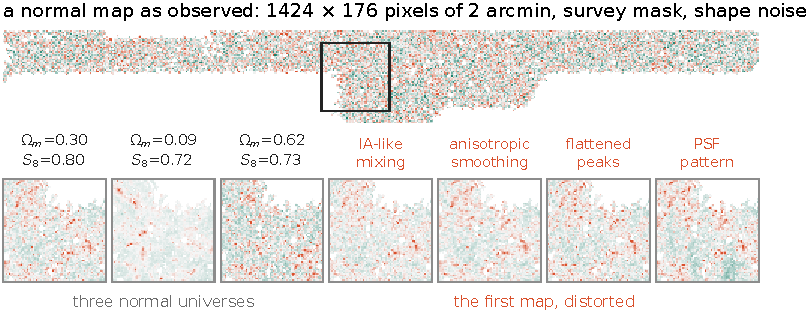
\includegraphics[width=\linewidth]{fig_maps.pdf}
\caption{\textbf{Normal universes differ more than distortions do.} Top: a normal test-like map (survey mask,
shape noise). Bottom: the same $128\times128$-pixel crop without noise, for three normal universes and for four of
my synthetic distortions of the first. Changing $\Omega_m$ changes the map far more than any of the distortions,
so a detector must judge a map against the universe that could have produced it.}
\label{fig:maps}
\end{figure}

% =================================================================================================
\section{Setup}

\paragraph{Data.} Each map covers $1424\times176$ pixels of 2 arcmin; 132,019 pixels lie inside the survey mask. I
add Gaussian shape noise ($\sigma=0.4/\sqrt{240}$ per pixel) to the clean training maps and round to float16, as in
the test files. The 25,856 training maps are 101 cosmologies $\times$ 256 realizations, and each realization index
carries the same baryon model $(T_{\mathrm{AGN}},f_0)$ in every cosmology. I therefore split at the level of maps,
not realizations: \emph{fit} (80\%) trains every model, \emph{calib} (10\%) sets every normalization, and
\emph{audit} (10\%) is held out for checks. A realization-level split would hold out whole baryon models.

\paragraph{Metric.} The score is the true-positive rate averaged over 100 false-positive rates, log-spaced in
$[0.001, 0.05]$. Since 59\% of these points lie below 1\%, the metric is decided by the few normal maps with the
highest scores. Much of my design aims to keep that tail of normal scores light.

% =================================================================================================
\section{Method}

\begin{figure}[t]
\centering
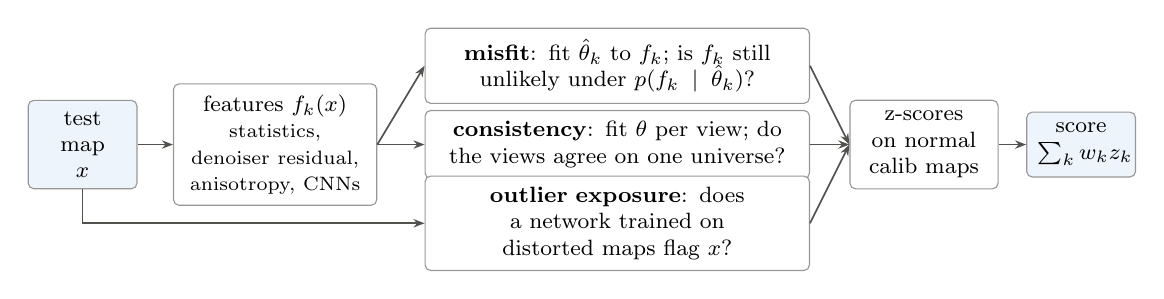
\begin{tikzpicture}[
  font=\footnotesize, >={Stealth[length=4pt]},
  box/.style={draw=cgray!60, rounded corners=2pt, align=center, inner sep=4pt, fill=white},
  test/.style={box, text width=4.6cm},
  arr/.style={->, cgray, line width=0.6pt}]
\node[box, fill=cbase, text width=1.1cm] (map) {test map\\$x$};
\node[box, right=0.45cm of map, text width=2.3cm] (feat) {features $f_k(x)$\\ \scriptsize statistics, denoiser
residual, anisotropy, CNNs};
\node[test, right=0.6cm of feat, yshift=1.0cm] (mis) {\textbf{misfit}: fit $\hat\theta_k$ to $f_k$; is $f_k$
still unlikely under $p(f_k\mid\hat\theta_k)$?};
\node[test, right=0.6cm of feat] (con) {\textbf{consistency}: fit $\theta$ per view; do the views agree on one
universe?};
\node[test, right=0.6cm of feat, yshift=-1.0cm] (oe) {\textbf{outlier exposure}: does a network trained on
distorted maps flag $x$?};
\node[box, right=0.5cm of con, text width=1.6cm] (z) {z-scores on normal calib maps};
\node[box, fill=cbase, right=0.35cm of z, text width=1.1cm] (s) {score\\$\sum_k w_k z_k$};
\draw[arr] (map) -- (feat);
\draw[arr] (feat.east) -- (mis.west);
\draw[arr] (feat.east) -- (con.west);
\draw[arr] (map.south) |- (oe.west);
\draw[arr] (mis.east) -- (z.west);
\draw[arr] (con.east) -- (z.west);
\draw[arr] (oe.east) -- (z.west);
\draw[arr] (z) -- (s);
\end{tikzpicture}
\caption{\textbf{Three tests of one question: can some normal universe explain this map?} Each test produces
z-scores calibrated on held-out normal maps; the OoD score is their weighted mean. Every step treats one map at a
time.}
\label{fig:method}
\end{figure}

\subsection{Misfit: the best-fitting universe}

For each family of features $f$ I learn the distribution of normal maps given their parameters, $p(f\mid\theta)$.
An MLP (3 layers of width 256) maps $\theta$ to a mean $\mu(\theta)$ and per-feature variances $\sigma^2(\theta)$,
trained by maximum likelihood on fit maps. The residuals $u=(f-\mu)/\sigma$ are not Gaussian and are strongly
correlated, so I model them with a Gaussian copula: each residual is mapped to a normal score through its
empirical quantiles, and their correlation is estimated with OAS shrinkage and an eigenvalue floor of 0.02. The
copula and the floor matter for the metric; without them a few normal maps reach very high misfit.

For a test map I fit $\theta$ by minimizing the negative log-likelihood, with a Gaussian prior on $\Delta z$
($\sigma=0.022$) and a soft penalty for leaving the region spanned by the training cosmologies (Adam, 150 steps,
three starts). The misfit is the copula energy at the fit, converted to a z-score with a location and scale that
depend smoothly on $\hat\theta$, both estimated on calib maps.

Five families serve as misfit members: difference-of-Gaussians wavelet norms (Sd); 112 statistics of the residual
$x-D(x)$ of a U-Net denoiser $D$ trained on normal maps (Dr), which isolate what the denoiser treats as noise; a noise battery of high-pass moments and tile variances (N2); the power spectrum with a binned bispectrum
(PsBh); and power-spectrum anisotropy (X), the log power in wedges $|k_x|>|k_y|$ versus $|k_y|>|k_x|$ per scale
band, aimed at PSF- and shear-like effects.

\subsection{Consistency: do the views agree?}

Fitting $\theta$ absorbs part of every distortion (Figure~\ref{fig:profiling}). But the fit to a distorted map is a
compromise, and different views of the map compromise differently: a small-scale suppression pulls a fit to
small-scale statistics but not one to large scales. I fit $\theta$ separately per view and measure how far the
estimates spread, as a Mahalanobis distance of their deviations from the mean, with mean and covariance taken from
calib maps. consP8 uses 8 views (two power-spectrum families, one-point PDF, extrema, Minkowski functionals, wavelet
norms, and a CNN's embedding and its direct $\theta$ prediction). consRplus uses 13 views (four scale bands, two CNN
embeddings and predictions, the denoiser families, and linear $\theta$ probes on the denoiser bottleneck and on the
anisotropy features). xSL fits small- and large-scale statistics separately and scores how much worse each fits at
the other's estimate.

\begin{figure}[t]
\centering
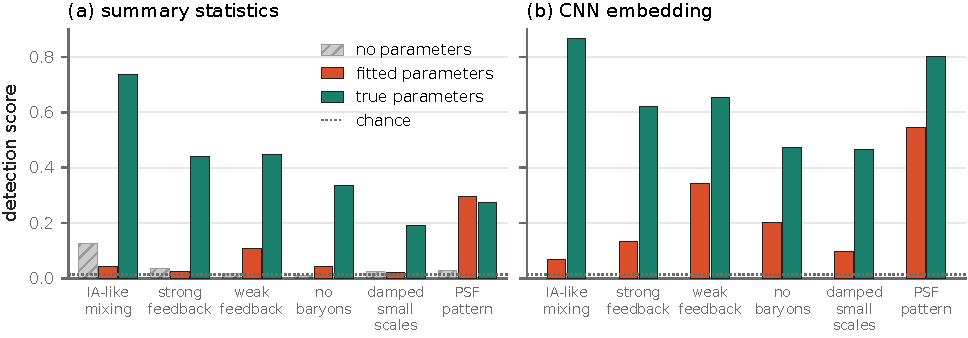
\includegraphics[width=\linewidth]{fig_profiling.pdf}
\caption{\textbf{The parameters make distortions visible, and fitting them hides the distortions again.} Detection
of six synthetic distortions on held-out maps by the misfit of (a) the 466 summary statistics and (b) a CNN
embedding. Without the parameters (gray) detection is near chance. With the true parameters (blue) it is high.
With fitted parameters (orange), as at test time, most of the gain is lost: the fit moves to a universe that
mimics the distortion. The consistency and outlier-exposure tests target this gap.}
\label{fig:profiling}
\end{figure}

\subsection{Outlier exposure: has the map been distorted?}

Some distortions are absorbed by every view, for instance an IA-like change that mimics a lower $S_8$ at all scales.
For these I train a CNN to tell normal maps from distorted ones. Distortions are drawn from 14 generator families
at log-uniform strengths, including shear and PSF errors, redshift-distribution errors, wrong noise levels and
masks, modified nonlinear and baryonic power, intrinsic alignments, source clustering and Poisson counts, and are
applied to clean fit maps before noise. The network also predicts the generator family and $\theta$, which shapes its features. Two members read it:
Ol is its OoD logit as a robust z-score on calib maps, and Oh is the misfit of its outputs under the likelihood
of the misfit test.

\subsection{Combining the tests}

Every member is a z-score with respect to normal calib maps, so the members share one scale. The final score is
the weighted mean $s=\sum_k w_k z_k / \sum_k w_k$ (Table~\ref{tab:weights}). The weights favor the consistency and
outlier-exposure members; the plain misfit of the base statistics (Sd) carries 3\% of the weight.

\begin{table}[t]
\centering\small
\begin{tabular}{llc@{\hspace{2.5em}}llc}
\toprule
member & test & weight & member & test & weight\\
\midrule
Dr   & misfit, denoiser residual     & 2.5 & consRplus & consistency, 13 views    & 3\\
X    & misfit, anisotropy            & 2   & xSL       & consistency, 2 scales    & 1\\
Sd   & misfit, wavelet norms         & 0.5 & consP8    & consistency, 8 views     & 0.5\\
N2   & misfit, noise battery         & 0.5 & Ol        & outlier exposure, logit  & 3\\
PsBh & misfit, spectrum + bispectrum & 0.5 & Oh        & outlier exposure, misfit & 1.5\\
\bottomrule
\end{tabular}
\caption{\textbf{Members and weights of the final score.} The consistency and outlier-exposure members carry 60\%
of the weight.}
\label{tab:weights}
\end{table}

\paragraph{One map at a time.} Every score is a function of its own map. Networks run in evaluation mode on
fixed-shape zero-padded batches, and each map is fitted independently. All normalizations were fixed on training
simulations; the test set is never used to fit, calibrate, normalize, rank or select anything. Leaderboard feedback
was used only to choose among submitted weightings.

% =================================================================================================
\section{Validation}

The test set's OoD maps come from distortions I do not know, so I validate on my own: 19 synthetic shifts of
normal maps (shear bias, smoothing, misestimated and non-Gaussian noise, small-scale suppression and boost, flattened
peaks, gradients, out-of-prior baryons, source clustering, Poisson counts, IA-like mixing, a PSF pattern).
Validating on audit maps proved misleading: all their cosmologies are seen in training, and it rated as equal two
weightings that the leaderboard separated by 0.08. The test maps' normal universes need not match the training
ones, so I hold out whole cosmologies instead: my \emph{leave-cosmology-out} proxy refits every member without 20
of the 101 cosmologies, in three disjoint sets, and scores the 19 shifts on the held-out maps.

The proxy ranked my main steps correctly (Figure~\ref{fig:results}b), but it is biased toward members built from
the same ideas as my shifts. Raising the weight of the outlier-exposure logit from 3 to 6 improved the proxy on
every fold and lowered the leaderboard by 0.004. I chose weights by the proxy and kept the leaderboard as the
final judge.

% =================================================================================================
\section{Results}

\begin{table}[t]
\centering\small
\begin{tabular}{lllc}
\toprule
submission & change & test added & public leaderboard\\
\midrule
start   & pipeline I started from & --- & 0.5253\\
v3-01   & new conditional likelihood, map-level splits & misfit & 0.5272 \dpos{+0.002}\\
v3-02   & + xSL, consP8 & consistency & 0.5669 \dpos{+0.040}\\
v3-04   & + denoiser residual; consistency at full weight & misfit, consistency & 0.6461 \dpos{+0.079}\\
v3-15b  & + more views, noise, bispectrum, anisotropy, Oh & all three & 0.6667 \dpos{+0.021}\\
v3-15d  & $-$ CNN-embedding misfit & --- & 0.6676 \dpos{+0.001}\\
\rowcolor{cbase} v3-16b & + Ol at weight 3 (final) & outlier exposure & \textbf{0.7037} \dpos{+0.036}\\
\midrule
v3-15g  & v3-15d without Oh & --- & 0.6479 \dneg{$-$0.020}\\
v3-16c  & v3-16b with Ol at weight 6 & --- & 0.6993 \dneg{$-$0.004}\\
\bottomrule
\end{tabular}
\caption{\textbf{Every test moved the leaderboard.} Public leaderboard score of each submission, with the change
from the row above (the two rows below the line are compared with v3-15d and v3-16b). Adding consistency was worth
0.040 on its first try; the denoiser residual with consistency at full weight, 0.079; the outlier-exposure network,
0.056 in total (Oh 0.020, Ol 0.036).}
\label{tab:lb}
\end{table}

\begin{figure}[t]
\centering
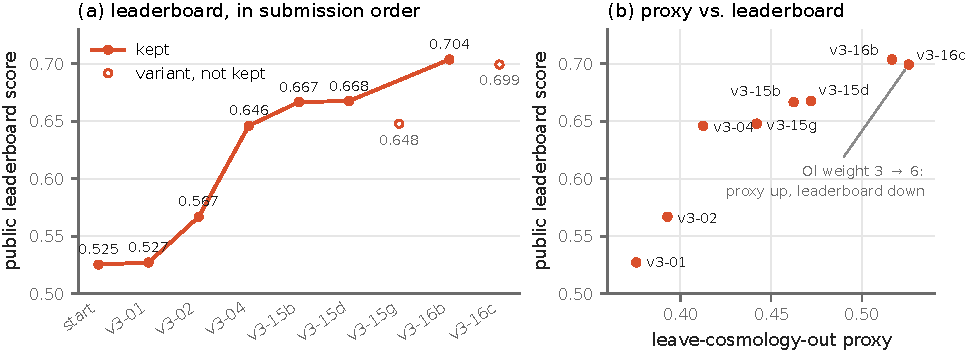
\includegraphics[width=\linewidth]{fig_results.pdf}
\caption{\textbf{Progress on the public leaderboard, and how far my proxy predicted it.} (a) Leaderboard score per
submission; open markers are variants I did not keep. (b) The leave-cosmology-out proxy orders the main steps
correctly but misses the last one.}
\label{fig:results}
\end{figure}

Table~\ref{tab:lb} lists every scored submission. The first rebuild of the likelihood alone barely moved the score
(0.5253 to 0.5272): a better misfit test, by itself, still lets the fit absorb the distortions. The consistency test
was the first large step, $+0.040$, and adding the denoiser residual with consistency at full weight gave the
largest, $+0.079$. Outlier exposure gave the final step. Removing its misfit member Oh costs 0.020, and adding its
logit Ol at weight 3 gains 0.036.

Interestingly, the leaderboard improved each time the plain misfit of the base statistics lost weight, from all of
the score in v3-01 to 3\% in the final weighting, and dropping the CNN-embedding misfit helped slightly ($+0.001$).
I read this as the test's normal maps sitting at universes my likelihoods fit less well than the training ones;
tests that compare a map with itself, or with distortions, are less exposed to that.

\paragraph{Compute.} Inference needs one GPU and PyTorch. Run with the organizers' ingestion program in their
runtime image on one A100 with 4 CPU cores, the package scores the 10,000 public test maps in 306~s with a peak of
7.6~GiB of GPU memory, and reproduces my leaderboard scores (Spearman correlation 0.9997). Training is modest; the
U-Net denoiser, for example, trains in 30 epochs on one A100.

% =================================================================================================
\section{Discussion}

Three limitations are worth stating. First, a distortion that is exactly degenerate with the parameters --- my
IA-like mixing --- passes both the misfit and the consistency tests; only outlier exposure sees it, and only when it
resembles something the network was trained on. Second, my validation shares its assumptions with my detector:
the synthetic shifts and the outlier-exposure generators come from the same list of plausible systematics, which is
why the proxy overrated the members built on them. A validation set of distortion types withheld from all design
choices would make the weights more trustworthy. Third, in my checks the highest-scoring normal maps come from
universes at the edge of the training range (low $\Omega_m$), where the fitted feedback parameters often sit on the
boundary and the outlier-exposure logit is also high. These maps set the low-FPR thresholds, so treating them better
would lift the metric directly.

The broader lesson is about where to look. Normal maps vary mostly along the directions of the five parameters, and
a detector that does not account for them sees mostly that variation. Conditioning on the parameters, and then
guarding against the fit that conditioning requires, turned summary statistics that are near chance on their own
into a detector that scores 0.70.

\end{document}
